% Content for Experimental Setup subsection
% This file is included in the main conference paper via % Content for Experimental Setup subsection
% This file is included in the main conference paper via % Content for Experimental Setup subsection
% This file is included in the main conference paper via % Content for Experimental Setup subsection
% This file is included in the main conference paper via \input{ExperimentalSetup}

To compare each transform, we chose 4 unique datasets all with different types of images. Sample images for all of the datasets can be seen in Fig. \ref{fig:datasetsamples}.
\begin{enumerate}
    \item \textbf{Kodak} - Includes general pictures of people and objects. We included this to test how each transform performed on normal images.
    \item \textbf{Aerial Images} - As the name suggests, contains images taken from the air of large sections of landscape. We expected many transforms like Haar and S+P to do well on these images because of their consistent global structure, 
    \item \textbf{Textures} - The inverse of Aerial Images, this includes close-up textures of a variety of surfaces and materials. This dataset is interesting because it includes some images with good global consistency, but also many images with much more sporadic textures that vary greatly even at a small scale.
    \item \textbf{Icons} - This includes low-resolution images of a variety of various digital icons. We chose this to test since the sharp edges and transitions in color challenge the transforms, especially those like DCT and DFT.
\end{enumerate}

\begin{figure}[!h] % [!h] is a common placement modifier (here, "force here if possible")
    \centering
    % --- Top Left Image (Subfigure a) ---
    \begin{subfigure}[b]{0.22\textwidth} % [b] aligns the subfigure baseline; 0.45\textwidth controls the width
        \centering
        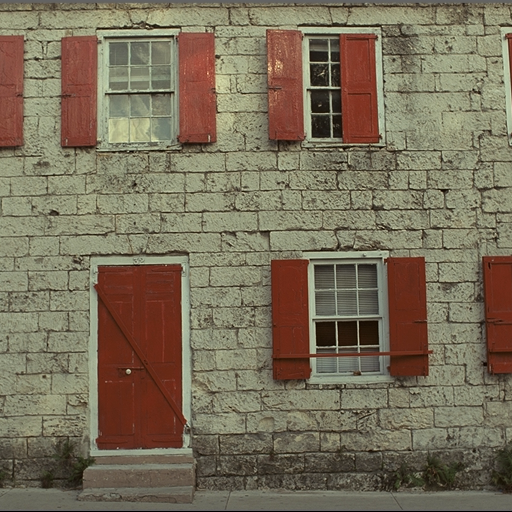
\includegraphics[width=\textwidth]{results/sample_images/kodak.png} % Replace image1.jpg with your file
        \caption{Sample \textbf{Kodak} image}
        \label{fig:kodakimg}
    \end{subfigure}
    \hfill % Adds horizontal space between the first two subfigures
    % --- Top Right Image (Subfigure b) ---
    \begin{subfigure}[b]{0.22\textwidth}
        \centering
        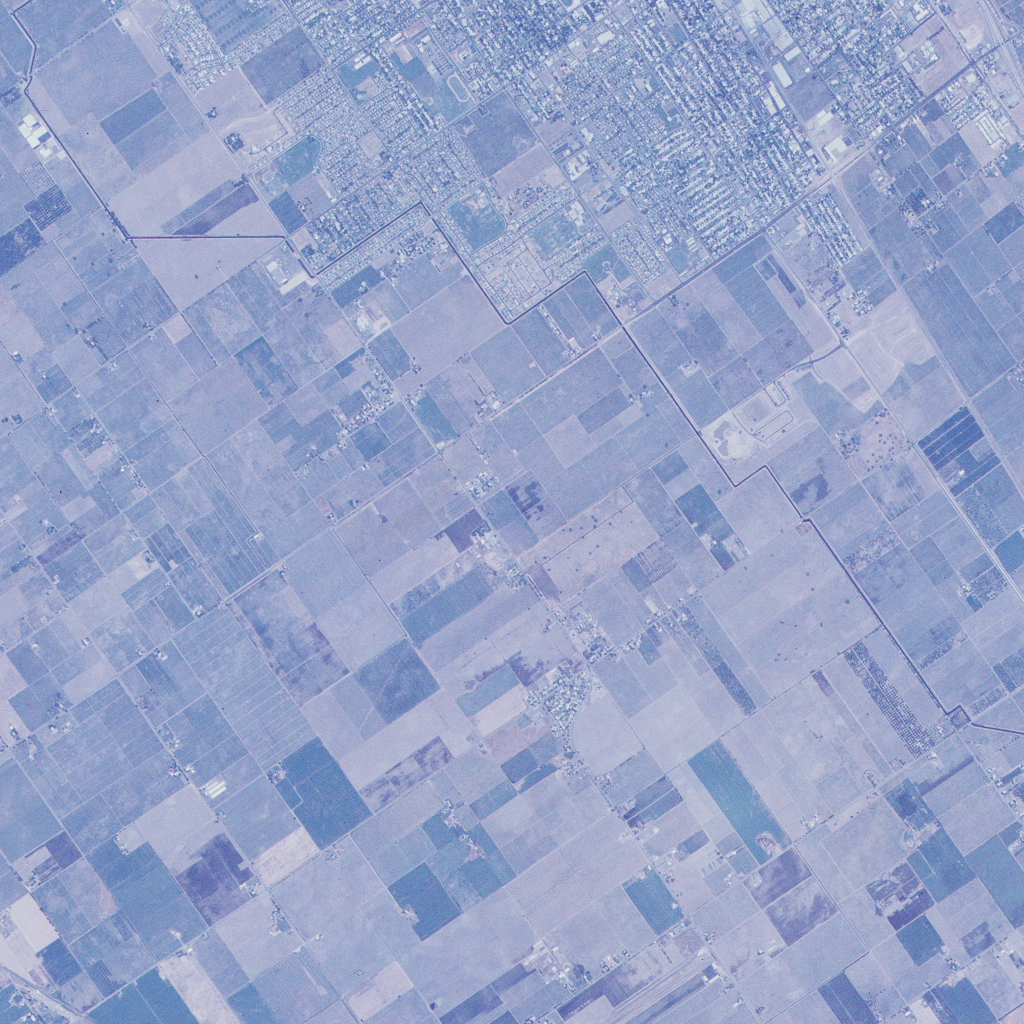
\includegraphics[width=\textwidth]{results/sample_images/aerial.png} % Replace image2.png with your file
        \caption{Sample \textbf{Aerial} image}
        \label{fig:aerialimg}
    \end{subfigure}
    
    \vspace{1em} % Adds vertical space between the top and bottom rows
    
    % --- Bottom Left Image (Subfigure c) ---
    \begin{subfigure}[b]{0.22\textwidth}
        \centering
        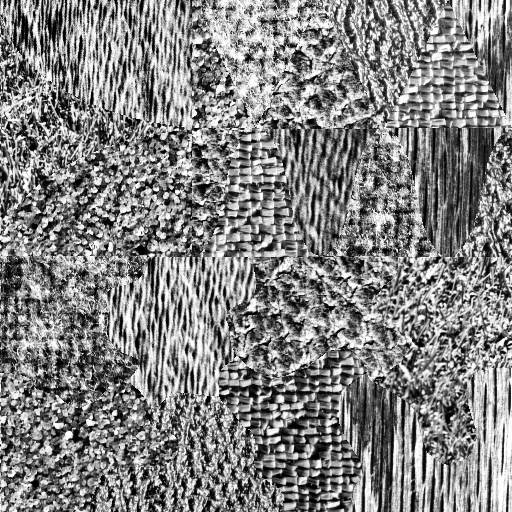
\includegraphics[width=\textwidth]{results/sample_images/texture.png} % Replace image3.eps with your file
        \caption{Sample \textbf{Texture} image}
        \label{fig:textureimg}
    \end{subfigure}
    \hfill
    % --- Bottom Right Image (Subfigure d) ---
    \begin{subfigure}[b]{0.22\textwidth}
        \centering
        
\includegraphics[width=\textwidth]{results/sample_images/icon.png} % Replace image4.gif with your file
        \caption{Sample \textbf{Icon} image}
        \label{fig:iconimg}
    \end{subfigure}
    
    % --- Main Caption for the entire 2x2 grid ---
    \caption{A sample image from each of the 4 datasets.}
    \label{fig:datasetsamples}
\end{figure}



To compare each transform, we chose 4 unique datasets all with different types of images. Sample images for all of the datasets can be seen in Fig. \ref{fig:datasetsamples}.
\begin{enumerate}
    \item \textbf{Kodak} - Includes general pictures of people and objects. We included this to test how each transform performed on normal images.
    \item \textbf{Aerial Images} - As the name suggests, contains images taken from the air of large sections of landscape. We expected many transforms like Haar and S+P to do well on these images because of their consistent global structure, 
    \item \textbf{Textures} - The inverse of Aerial Images, this includes close-up textures of a variety of surfaces and materials. This dataset is interesting because it includes some images with good global consistency, but also many images with much more sporadic textures that vary greatly even at a small scale.
    \item \textbf{Icons} - This includes low-resolution images of a variety of various digital icons. We chose this to test since the sharp edges and transitions in color challenge the transforms, especially those like DCT and DFT.
\end{enumerate}

\begin{figure}[!h] % [!h] is a common placement modifier (here, "force here if possible")
    \centering
    % --- Top Left Image (Subfigure a) ---
    \begin{subfigure}[b]{0.22\textwidth} % [b] aligns the subfigure baseline; 0.45\textwidth controls the width
        \centering
        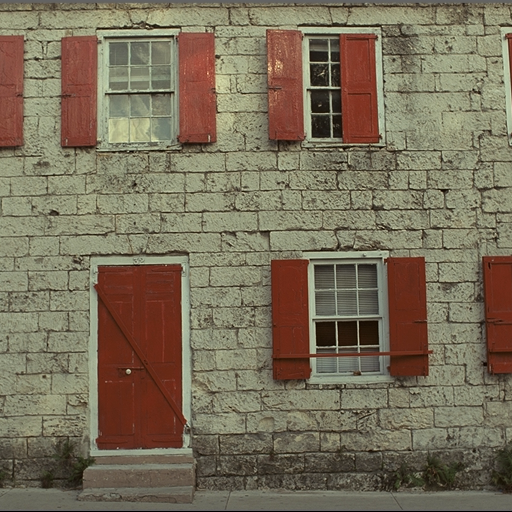
\includegraphics[width=\textwidth]{results/sample_images/kodak.png} % Replace image1.jpg with your file
        \caption{Sample \textbf{Kodak} image}
        \label{fig:kodakimg}
    \end{subfigure}
    \hfill % Adds horizontal space between the first two subfigures
    % --- Top Right Image (Subfigure b) ---
    \begin{subfigure}[b]{0.22\textwidth}
        \centering
        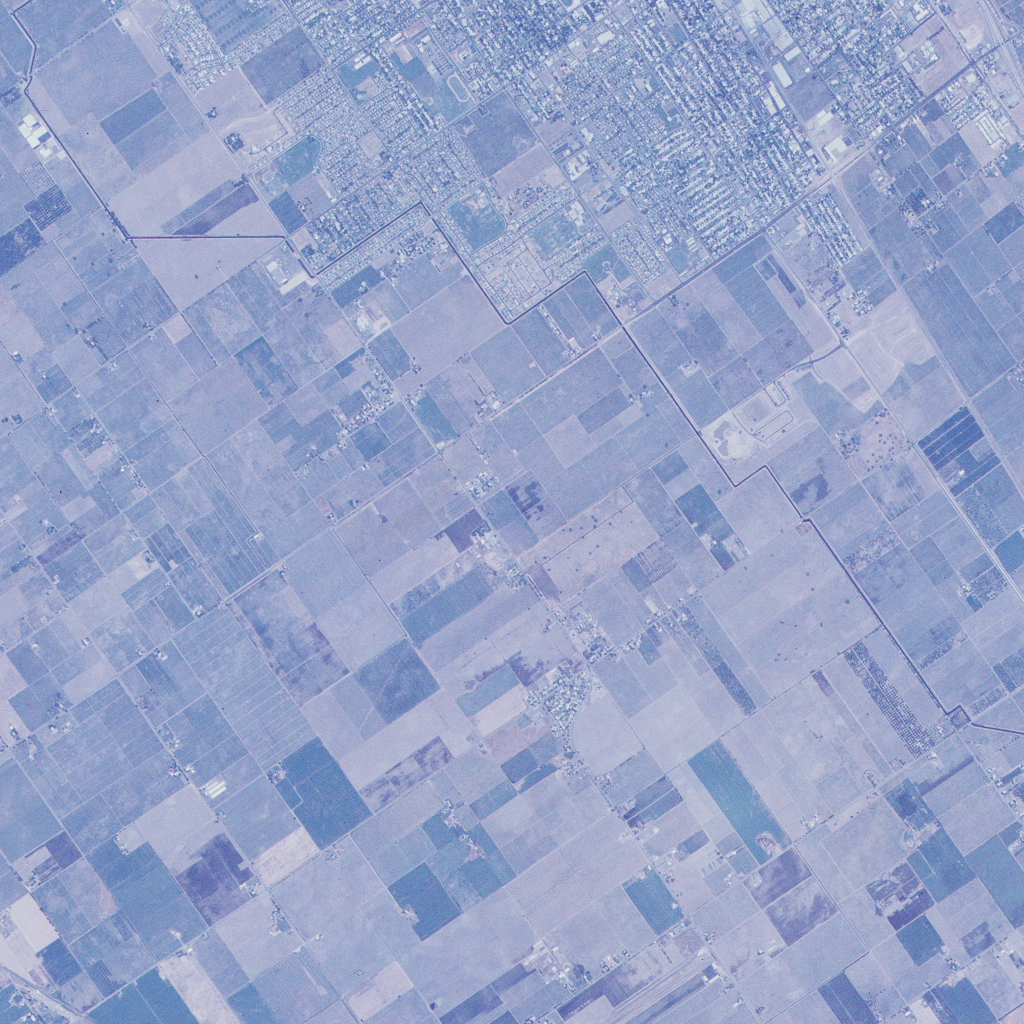
\includegraphics[width=\textwidth]{results/sample_images/aerial.png} % Replace image2.png with your file
        \caption{Sample \textbf{Aerial} image}
        \label{fig:aerialimg}
    \end{subfigure}
    
    \vspace{1em} % Adds vertical space between the top and bottom rows
    
    % --- Bottom Left Image (Subfigure c) ---
    \begin{subfigure}[b]{0.22\textwidth}
        \centering
        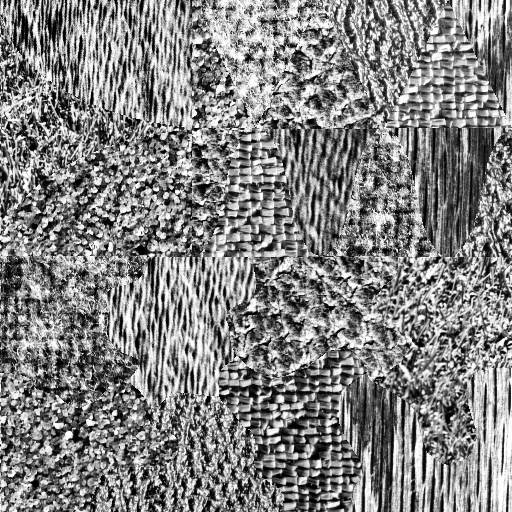
\includegraphics[width=\textwidth]{results/sample_images/texture.png} % Replace image3.eps with your file
        \caption{Sample \textbf{Texture} image}
        \label{fig:textureimg}
    \end{subfigure}
    \hfill
    % --- Bottom Right Image (Subfigure d) ---
    \begin{subfigure}[b]{0.22\textwidth}
        \centering
        
\includegraphics[width=\textwidth]{results/sample_images/icon.png} % Replace image4.gif with your file
        \caption{Sample \textbf{Icon} image}
        \label{fig:iconimg}
    \end{subfigure}
    
    % --- Main Caption for the entire 2x2 grid ---
    \caption{A sample image from each of the 4 datasets.}
    \label{fig:datasetsamples}
\end{figure}



To compare each transform, we chose 4 unique datasets all with different types of images. Sample images for all of the datasets can be seen in Fig. \ref{fig:datasetsamples}.
\begin{enumerate}
    \item \textbf{Kodak} - Includes general pictures of people and objects. We included this to test how each transform performed on normal images.
    \item \textbf{Aerial Images} - As the name suggests, contains images taken from the air of large sections of landscape. We expected many transforms like Haar and S+P to do well on these images because of their consistent global structure, 
    \item \textbf{Textures} - The inverse of Aerial Images, this includes close-up textures of a variety of surfaces and materials. This dataset is interesting because it includes some images with good global consistency, but also many images with much more sporadic textures that vary greatly even at a small scale.
    \item \textbf{Icons} - This includes low-resolution images of a variety of various digital icons. We chose this to test since the sharp edges and transitions in color challenge the transforms, especially those like DCT and DFT.
\end{enumerate}

\begin{figure}[!h] % [!h] is a common placement modifier (here, "force here if possible")
    \centering
    % --- Top Left Image (Subfigure a) ---
    \begin{subfigure}[b]{0.22\textwidth} % [b] aligns the subfigure baseline; 0.45\textwidth controls the width
        \centering
        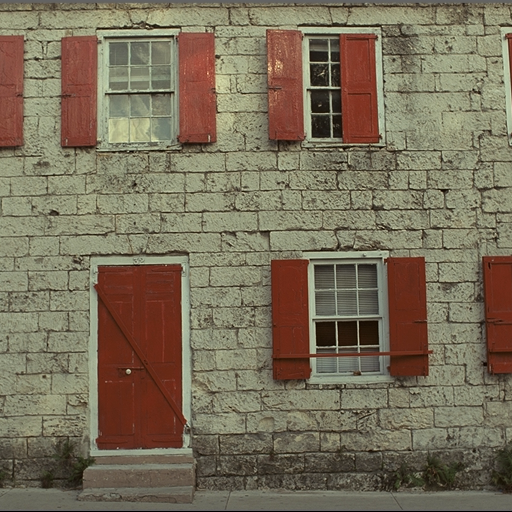
\includegraphics[width=\textwidth]{results/sample_images/kodak.png} % Replace image1.jpg with your file
        \caption{Sample \textbf{Kodak} image}
        \label{fig:kodakimg}
    \end{subfigure}
    \hfill % Adds horizontal space between the first two subfigures
    % --- Top Right Image (Subfigure b) ---
    \begin{subfigure}[b]{0.22\textwidth}
        \centering
        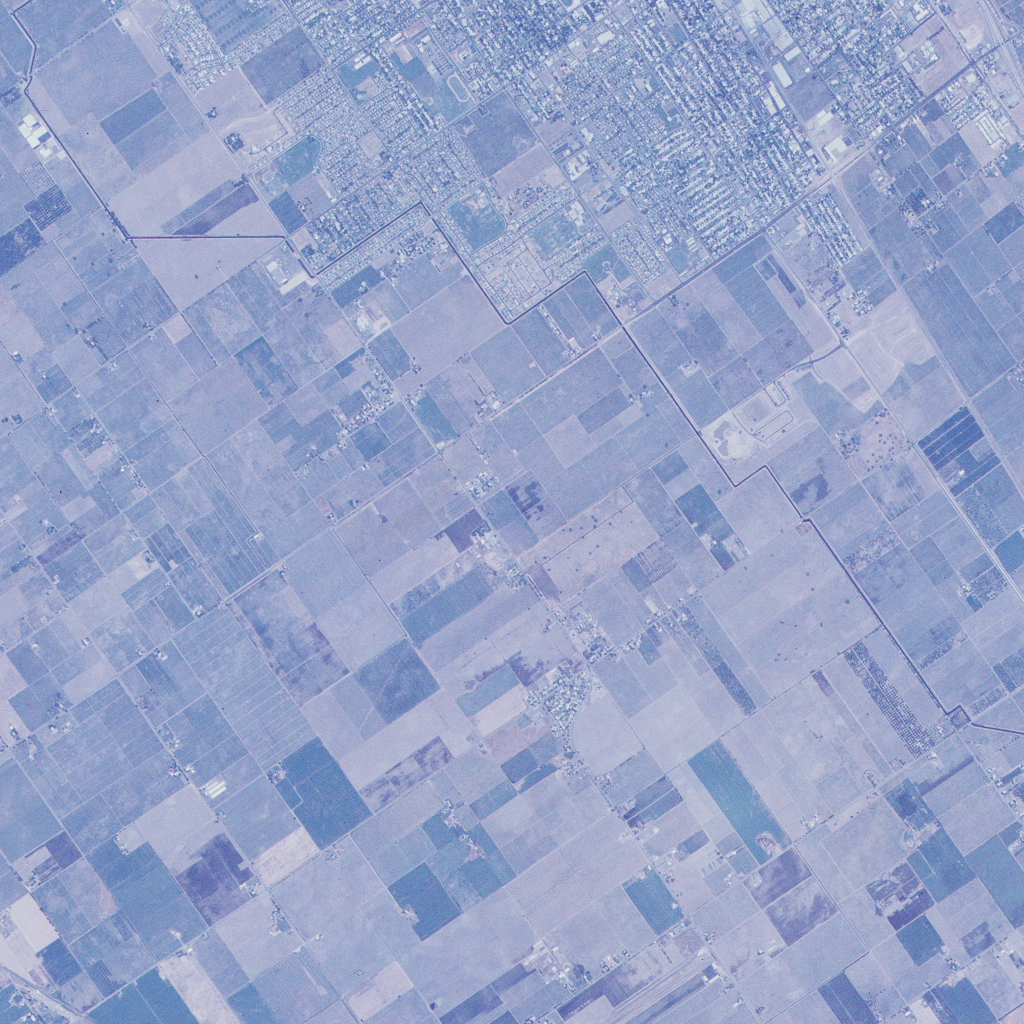
\includegraphics[width=\textwidth]{results/sample_images/aerial.png} % Replace image2.png with your file
        \caption{Sample \textbf{Aerial} image}
        \label{fig:aerialimg}
    \end{subfigure}
    
    \vspace{1em} % Adds vertical space between the top and bottom rows
    
    % --- Bottom Left Image (Subfigure c) ---
    \begin{subfigure}[b]{0.22\textwidth}
        \centering
        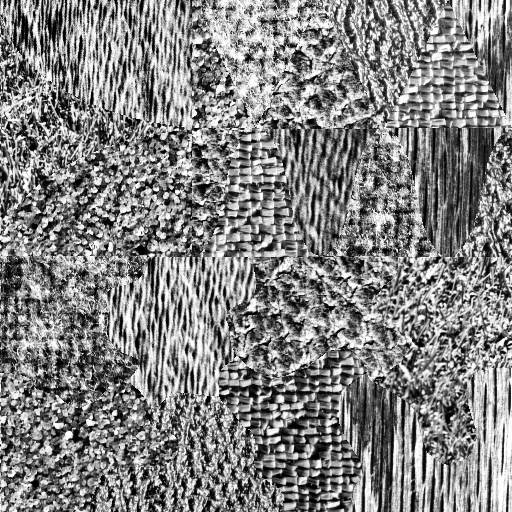
\includegraphics[width=\textwidth]{results/sample_images/texture.png} % Replace image3.eps with your file
        \caption{Sample \textbf{Texture} image}
        \label{fig:textureimg}
    \end{subfigure}
    \hfill
    % --- Bottom Right Image (Subfigure d) ---
    \begin{subfigure}[b]{0.22\textwidth}
        \centering
        
\includegraphics[width=\textwidth]{results/sample_images/icon.png} % Replace image4.gif with your file
        \caption{Sample \textbf{Icon} image}
        \label{fig:iconimg}
    \end{subfigure}
    
    % --- Main Caption for the entire 2x2 grid ---
    \caption{A sample image from each of the 4 datasets.}
    \label{fig:datasetsamples}
\end{figure}



To compare each transform, we chose 4 unique datasets all with different types of images. Sample images for all of the datasets can be seen in Fig. \ref{fig:datasetsamples}.
\begin{enumerate}
    \item \textbf{Kodak} - Includes general pictures of people and objects. We included this to test how each transform performed on normal images.
    \item \textbf{Aerial Images} - As the name suggests, contains images taken from the air of large sections of landscape. We expected many transforms like Haar and S+P to do well on these images because of their consistent global structure, 
    \item \textbf{Textures} - The inverse of Aerial Images, this includes close-up textures of a variety of surfaces and materials. This dataset is interesting because it includes some images with good global consistency, but also many images with much more sporadic textures that vary greatly even at a small scale.
    \item \textbf{Icons} - This includes low-resolution images of a variety of various digital icons. We chose this to test since the sharp edges and transitions in color challenge the transforms, especially those like DCT and DFT.
\end{enumerate}

\begin{figure}[!h] % [!h] is a common placement modifier (here, "force here if possible")
    \centering
    % --- Top Left Image (Subfigure a) ---
    \begin{subfigure}[b]{0.22\textwidth} % [b] aligns the subfigure baseline; 0.45\textwidth controls the width
        \centering
        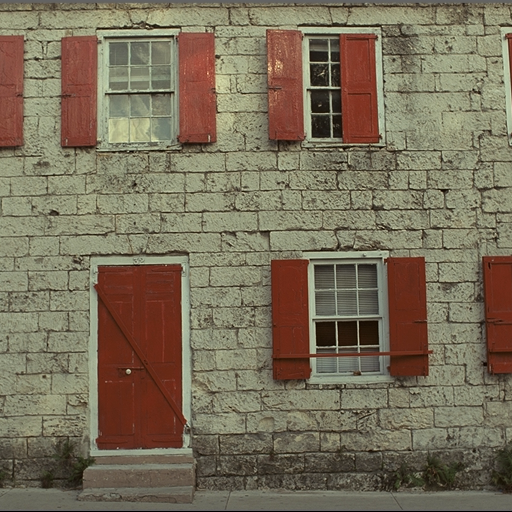
\includegraphics[width=\textwidth]{results/sample_images/kodak.png} % Replace image1.jpg with your file
        \caption{Sample \textbf{Kodak} image}
        \label{fig:kodakimg}
    \end{subfigure}
    \hfill % Adds horizontal space between the first two subfigures
    % --- Top Right Image (Subfigure b) ---
    \begin{subfigure}[b]{0.22\textwidth}
        \centering
        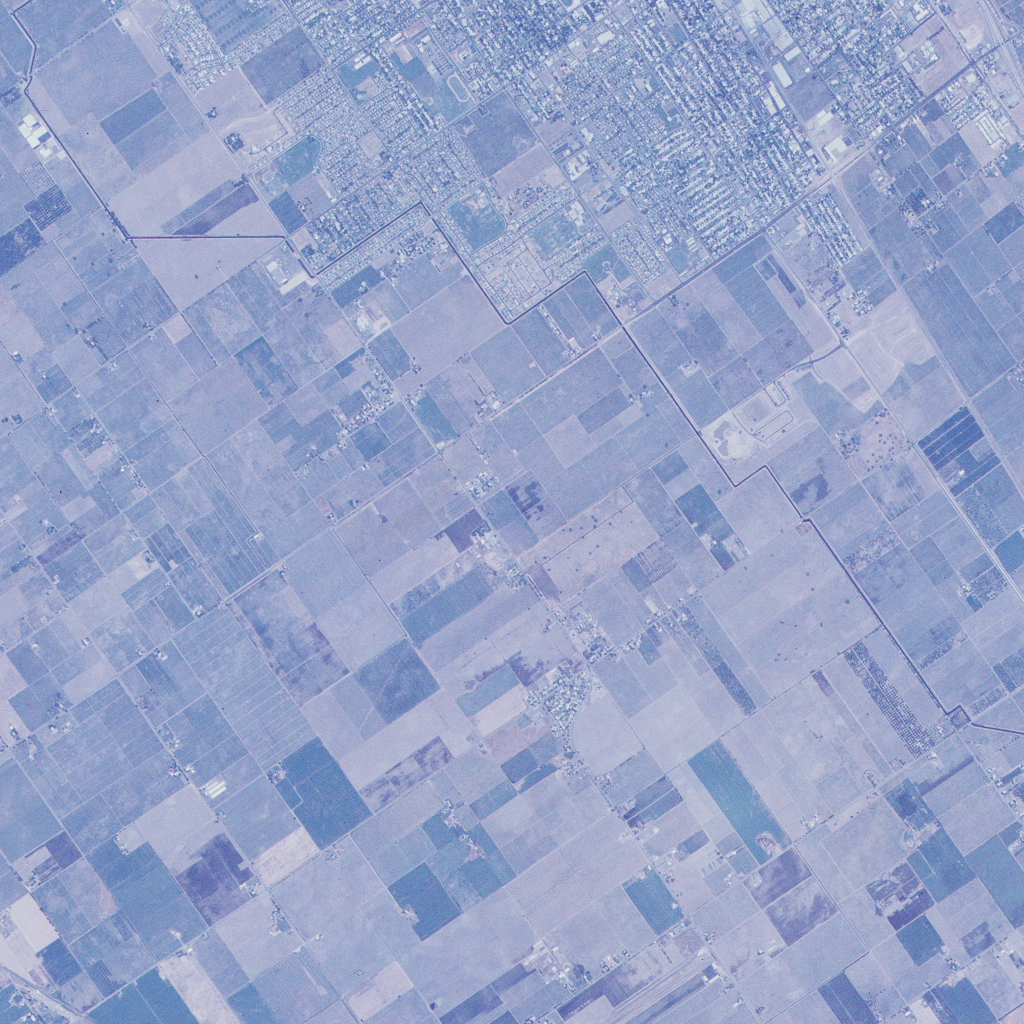
\includegraphics[width=\textwidth]{results/sample_images/aerial.png} % Replace image2.png with your file
        \caption{Sample \textbf{Aerial} image}
        \label{fig:aerialimg}
    \end{subfigure}
    
    \vspace{1em} % Adds vertical space between the top and bottom rows
    
    % --- Bottom Left Image (Subfigure c) ---
    \begin{subfigure}[b]{0.22\textwidth}
        \centering
        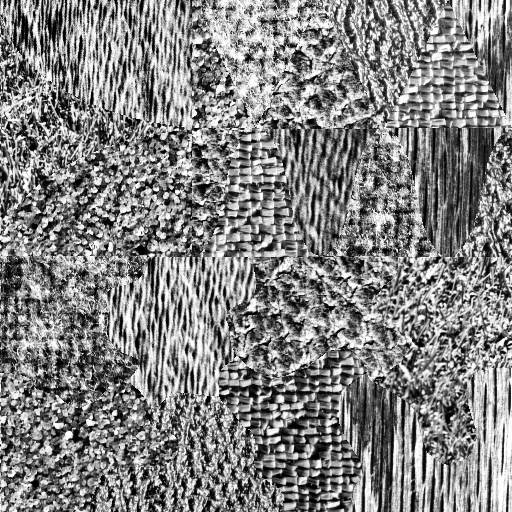
\includegraphics[width=\textwidth]{results/sample_images/texture.png} % Replace image3.eps with your file
        \caption{Sample \textbf{Texture} image}
        \label{fig:textureimg}
    \end{subfigure}
    \hfill
    % --- Bottom Right Image (Subfigure d) ---
    \begin{subfigure}[b]{0.22\textwidth}
        \centering
        
\includegraphics[width=\textwidth]{results/sample_images/icon.png} % Replace image4.gif with your file
        \caption{Sample \textbf{Icon} image}
        \label{fig:iconimg}
    \end{subfigure}
    
    % --- Main Caption for the entire 2x2 grid ---
    \caption{A sample image from each of the 4 datasets.}
    \label{fig:datasetsamples}
\end{figure}

